\chapter{Methodology of Added Features}

	\section{Metric Builder}

		\subsection{Back End}

			For the Metric Builder the first question we have to address is how to model, store and compute a user metric.
			We distinguish between the following two options:

			\begin{enumerate}[itemsep=-1.5mm]
				\item
					Precompute and then store the user metric value for each metric in the database
					\begin{itemize}[itemsep=-1.5mm]
						\item
							Pros
							\begin{itemize}
								\item
									Fast to retrieve; no computation needed 
									no computation needed
							\end{itemize}
						\item
							Cons
							\begin{itemize}
								\item
									Waste of space in the database
								\item
									User metric data remains static;
									update in the underlying data does not cause an update in the user metric
							\end{itemize}
					\end{itemize}
				\item
					Store a user metric as a metadata only, in the form of a derivation formula, and compute values on-the-fly (on-demand)
					\begin{itemize}[itemsep=-1.5mm]
						\item
							Pros
							\begin{itemize}
								\item
									Efficient use of the database space
								\item
									User metric data is always in sync with underlying data
							\end{itemize}
						\item
							Cons
							\begin{itemize}
								\item
									Might be time-consuming to compute
							\end{itemize}
					\end{itemize}
			\end{enumerate}

			Looking at the cons of each option, we attempted to approximate how bad they are.
			Having $n$ users each creating $m$ user metrics each of which has data for $k$ years
			we have $m \cdot n \cdot k \cdot 50$ entries in the database.
			This data would be a snapshot. If any data point in the metrics changes, user metrics remain out of sync.

			For the second option, it was difficult to approximate time it takes to compute a user metric 
			as it depends on the server load and the number of metrics involved in the user metric. 
			We implemented the second option and benchmarked it with $3$ users trying to compute 
			largest possible user metric (all metrics with all states selected). 
			It took around $1.5$ seconds to load all $3$ user metrics. 
			This drove our design decision towards the second option - computing metrics on-the-fly.
			
			\subsubsection{Note on normalization and missing values}
			
				The basic formula for the user metric is
				
				\[
					V_y = \frac{ \sum_{i \in I} v_{iy} \cdot c_i }{100} 
				\]
				
				where:
				\begin{itemize}
					\item
						$V_y$ is the value of the user metric for the year $y$
					\item 
						$I$ is a set of metrics in the user metric
					\item
						$v_{iy}$ is a value of $i_\text{th}$ metric for the year
						$y$
					\item
						$c_i$ is a user defined coefficient of $i_{\text{th}}$ 
						metric ($c \in [0, 100]$) 
				\end{itemize}
				
				However, this does not account for the different magnitudes of different metrics. For example, one metric could be a population and be measured in hundreds of millions, the other one could be taxes, and be measured in percents. If we simply take the average of values in these two metrics, it would not make sense as the value of the higher scale metric (population) will take over the value of the lower scale metric (taxes).

				This problem is solved with \emph{normalization} - adjusting values measured on different scales to a notionally common scale.
				
				We used \emph{z-transform} method to normalize data in the user metric. For each year and metric, normalized piece has the following form.
				
				\[
					\text{value}_\text{normalized} = \frac{\text{value}_\text{denormalized} - \text{mean}}{\text{standard deviation}}
				\]
				
				This way we can put together metrics of different scales.
				
				The other decision we had to make was about missing values. Different metrics may have values only for certain years. We decided to take the closest older value for the missing year. If there are no values prior to the missing year, we use the oldest value. 

		\subsection{Front End}
		
			The main goals for the front end of the Metric Builder feature was to design a webpage 
			that was easy to use, easily accessible, intuitive, and consistent 
			with the design of other pages on the MATTERS site. 
			The Metric Builder feature needed to be a tool that allowed users with any level of 
			technological background to easily build their metric formula from preexisting metrics, 
			assign weights to their chosen metrics, and be able to make changes to their metric formula at any time.
			
			The front end for the Metric Builder page was created through the use of HTML, CSS and JavaScript. 
			To make the page consistent with the rest of the site, code was reused from the Data Explorer page. 
			The Data Explorer page, as seen in Figure \ref{fig:dataexplorer}, within MATTERS allows users to select 
			preexisting metrics (from the left dropdown menus) to then visualize this on the site in multiple different visual display types, 
			including a bar chart, line graph, heat map, or table, by selecting the display type on the right side of the black bar via an icon. The framework for the 
			Data Explorer was the page most similar to how we wanted the Metric Builder to look like. Thus we opted to 
			reuse and modify code from that page to create our new feature. 
			
			\begin{figure}[t]
				\centering
					\fbox{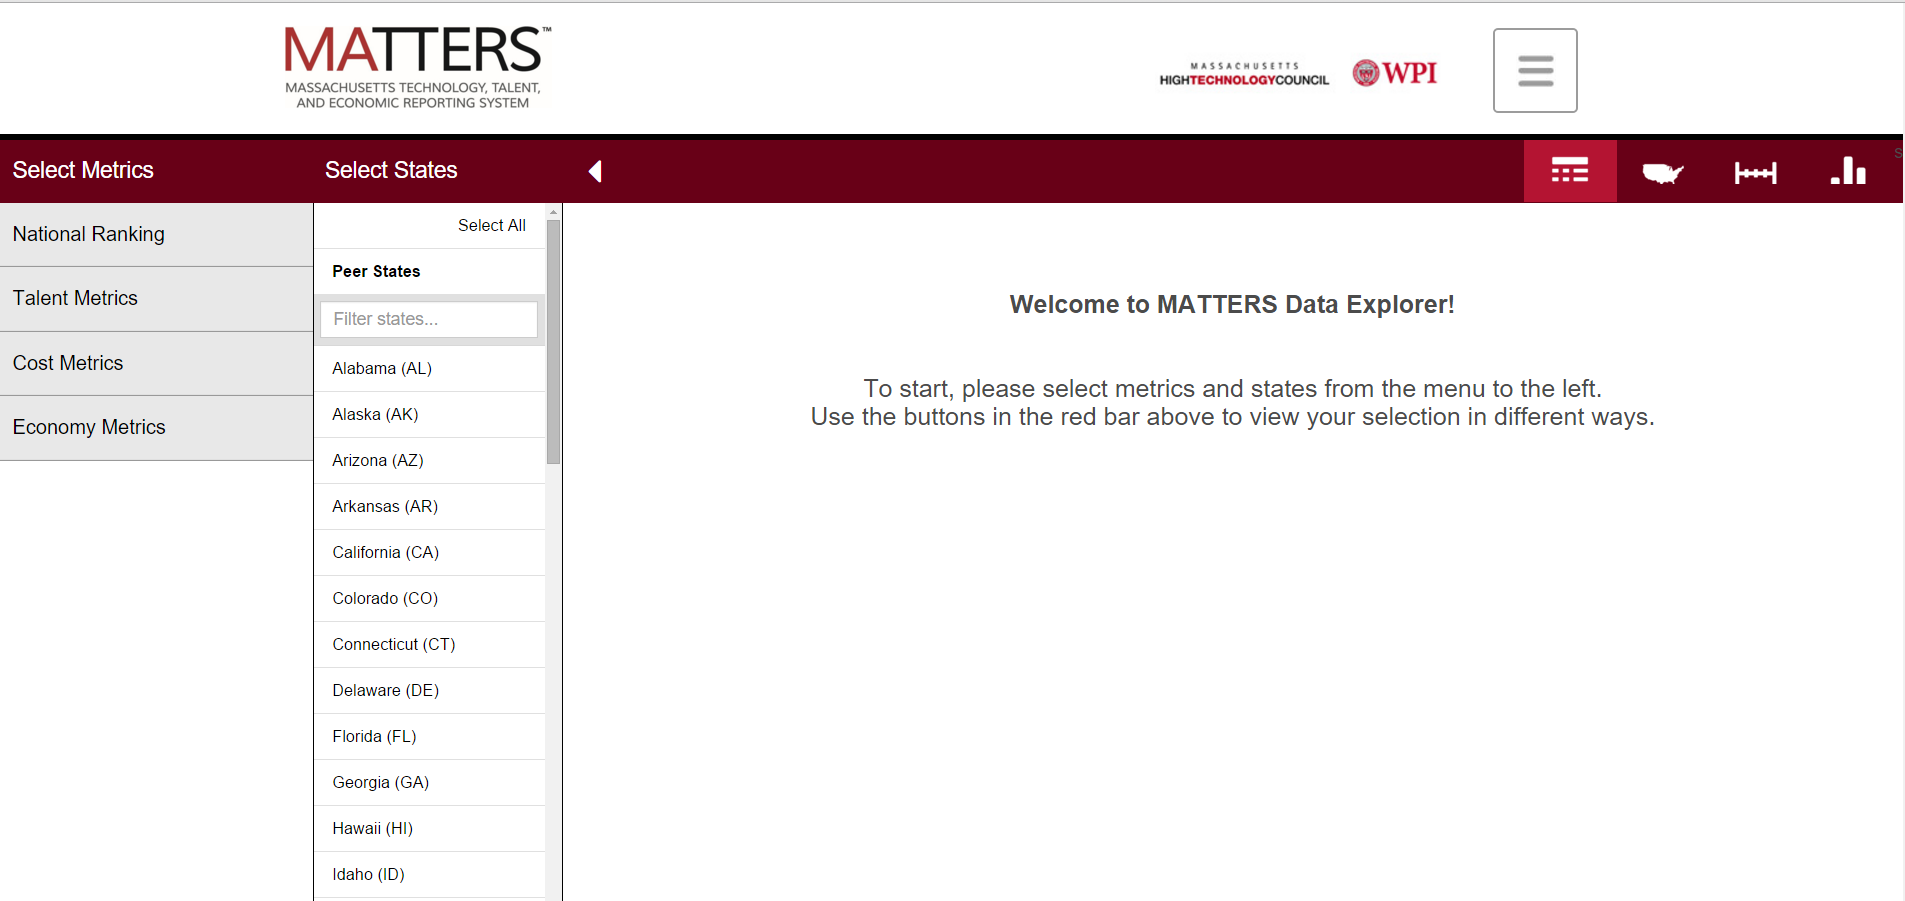
\includegraphics[width=0.75\textwidth]{images/dataexplorer.png}}
					\caption{Data Explorer Page}
				\label{fig:dataexplorer}
			\end{figure}
			
			The Data Explorer page allows users to select metrics and states that they would like to view through the use of the left sidebar (See Figure \ref{fig:dataexplorer}). 
			Because the intended users for the Metric Builder feature are meant to be authorized users with 
			experience using the MATTERS Data Explorer, we used the sidebar from the Data Explorer as the 
			basis for how the users would select their metrics on the Metric Builder page as well. Since the Metric Builder does not need a user to select states, 
			that part of the sidebar was removed. We also removed rankings from the metric selection column of the sidebar since rankings are manipulations of 
			various other metrics already found in the database. 
			
			Once a user selects the metrics they wish to use in order to create their own metric formula, they have the ability to assign each of them different weights 
			to decide how much of a factor each of the metric's data will be in the formula. To adjust the weight of a metric, users can use the sliders that appear under 
			each metric that they have selected. The sliders work horizontally from left to right and allow a weight from zero (which would be the same as not including the metric) 
			to one hundred. Users can click on a section of the slider to move to that weight, click and drag to a specific weight or use the arrow keys to move the slider's value up or down. 
			The idea for the sliders came from a New York Times site which allows users to interactively calculate their rent and other values using visual sliders \cite{slider}. The sliders are 
			visually appealing and simple to use and understand.
			
			The Metric Builder displays options to name the user's custom metric, save their metric and also go back and edit or delete the metric they have created. There is a 
			simple to use button that says "Remove" next to each metric chosen, making it easy for users to change the metrics included in their formula. The input 
			box to name the custom metric and save the changes can be found below all of the chosen metrics and sliders. This was done to help users and encourage them to 
			properly weigh all the selected metrics before leaving saving their custom metric formula to use, as users typically look at a webpage from top to bottom.
		
			Finally, above all of the metrics selected is a box displaying the basics of their created metric formula. As the users update metric selections and their various weights,
			the formula will update and show the basics of the math that needs to be done on the back end. This includes showing the users that they are 
			multiplying each data point by the chosen weight before adding each metric's data values together, and that sum is being divided by the total weight as a weighted average approach. 
			This is shown in a simple way to make sure that users can follow along and are aware of exactly what they changing when they adjust their formulas. 
			Once content, each time a user saves and updates their formula they will be prompted and subsequently directed to the Data Explorer page where they can begin using their custom metrics and displaying the data with the various visualization options.
			

	\section{API}
			
			Implementing an API, there are several design decisions to consider, including:
			\begin{itemize}
				\item
					Do we implement a closed API or open API? 
					If closed, how do we implement authentication.
				\item
					Which methods do we support via this API?
				\item
			        What is the syntax of the query string? 	
				\item
				    What is the output format?
			\end{itemize}
			
			\subsection{Authentication}
				
				Although MATTERS system is a public resource, 
				we decided we would like the ability to track users of our API, how and how often. 
				This requirement made us chose a closed API option. 
				Thinking of authentication, we had a few options, including:
				
				\begin{itemize}
					\item
						Bind to a particular user
					\item
						Simple \emph{API key} (token) authentication
					\item
						Complex \emph{handshake} mechanism					
					\item
						\emph{Handshake} mechanism with random value
				\end{itemize}
				
				Binding to API user t regular user would allow any registered user to access API. 
				Although this kind of authentication is the easiest one to implement we wanted a separate API users.
				
				Simple  \emph{API key} authentication is the one when API users are given unique token 
				(long random string) which they need to provide with each request. 
				Based on this token system is able to accept or deny connection and track individual users.
				
				\emph{Handshake} mechanism with random value involves the following steps
				
				% source http://web.cs.wpi.edu/~cs4513/c16/projects/proj2/index.html
				\begin{itemize}
					\item
						Client sends in username (not password)
					\item
						Server responds by sending back unique random number
					\item
						Client encrypts using user's password plus number as key
					\item
						Client sends hashed or encrypted value back to server
					\item
						Server encrypts using the user's same password plus number as key
					\item
						Server compares two hashed or encrypted values, if same then grant access
				\end{itemize}
				
				Provided that the main purpose of the API being closed is tracking an activity 
				for statistical purposes, \emph{API key} authentication was implemented.
				The user has to apply for this key separately of creating a regular account.
				The key will uniquely identify the user. If user forgets the key, 
				he or she can recover it through the email.

			\subsection{Methods}
				
				Main method implemented in the API is \code{api/data?}. 
				This method returns all data points for given metrics, states and years.
				
				Since \code{api/data?} needs specific IDs as arguments, there is a need for supporting 
				methods which show information about metrics and states. 
				So we also implemented \code{api/metrics?} and \code{api/states?}.

			\subsection{Query string and output format}
			
				The are two options for constructing a query string, namely:
				\begin{itemize}
					\item
						\code{api/method?argument1=value1\&argument2=value2\&...}
					\item
						\code{api/method/value1/value2/...}
				\end{itemize}
				
				To make out API user-friendly, we chose to implement the first option since it clearly 
				shows which value corresponds to which argument. Furthermore, these argument-value pairs may be in any order. 
				Lastly, arguments that have no value can be omitted.
				
				The final query strings are given is Listing \ref{apicode}. See
				Appendix \ref{app:apidoc} for an extensive documentation of the
				API.
				
				\begin{lstlisting}[
					frame=lines,
					caption={API methods examples}, 
					label=apicode, 
					backgroundcolor=\color{codegray}, 
					emph={data,metrics, states},
					emphstyle=\underbar
				]
/* method */
/api/data?metric=&state=&year=&apiKey=
/* example */
/api/data?metric={16,32}&state=MA&year=*&apiKey=key

/* method */
/api/metrics?apiKey=
/* example */
/api/metrics?apiKey=key

/* method */
/api/states?apiKey=
/* example */
/api/states?apiKey=key
				\end{lstlisting}
				
				The output format JSON (JavaScript Object Notation) was chosen
				as it both comapact and human and computer readable. 
				
			\subsection{Documentation}
				
				In order for the developers to know how to make proper API calls, 
				it was necessary to create the API Documentation page for MATTERS. 
				The documentation providers users with full information on the MATTERS API 
				and how to use it, as well as examples of valid API calls and the output 
				that they would return. It is important to ensure that the API Documentation 
				is free of both natural language and code sample errors, as this tool is 
				what developers unfamiliar with using the API rely on to understand how 
				to properly access and extract data \cite{errors}. 
				
				In order to make the documentation easy to follow, the documentation was divided into sections. 
				The main sections of the API Documentation were: an overview, the methods, 
				the parameters, and examples. The layout of the MATTERS API Documentation was based on the 
				API Documentation of Tradestation, which had was very simple and easy to follow \cite{apiex}. 
				The Tradestation documentation provided a summary, path, parameters, and examples of both an 
				API call and what it would return. An example of their documentation can be found at: 
				http://tradestation.github.io/webapi-docs/en/users/accounts/ \cite{apiex}. For the MATTERS API, 
				it was necessary to include information on how to retrieve a user's API key. 
				Further we described the proper format to get the data desired for different, years, states, 
				and metrics. The API Documentation sections are explained in the following sections below. 
				The final, complete API Documentation can be found in Appendix 1.
				
				
			\subsubsection{Overview of the API}
				
				The API Documentation begins with a summary about what the MATTERS API is and what 
				data points the API tool gives users access to. This section also includes an 
				interactive table of contents which allows users to quickly navigate to a specific 
				section of the documentation to look for information. This allows users to easily 
				find what they are looking for without having to scroll through the entire 
				documentation page. It provides a brief overview of everything that follows.
				
			\subsubsection{API Key Subsection}
				
				Developers without authorization do not have the ability to use the MATTERS API 
				until they have been given an API key. These users are directed to the “Contact Us” 
				page of the MATTERS site in order to send an email request to become an authorized user with their own key. 
				This section also explains that the API key is used in all 
				API calls in order to validate the user's request.
				
			\subsubsection{States Subsection}
				
				In this section, users are instructed on the proper format needed to retrieve a single state, 
				list of states, or all states. If a user does not know any other information 
				regarding the states in the MATTERS system, they are shown where to find the relevant
				information needed via an API request.
				
			\subsubsection{Metrics Subsection}
				
				In this section, users are given the proper format in order to request data for a single metric, 
				list of metrics or all metrics in the MATTERS data warehouse. The documentation explains 
				that in order to access data from metrics, the metric parameter values must be the 
				proper metric's ID number. The user is also given the path to all information 
				regarding the metrics, which will give the user the metric names, ID numbers and details.
				
			\subsubsection{Years Subsection}
				
				Users are given the proper format to request data from specific years. 
				Users may request data for a single year, range of years or all years in the MATTERS data warehouse. 
				
			\subsubsection{Examples of API Calls}
				
				Following the parameters and methods of the MATTERS API, the documentation provides 
				the users with two examples of valid API requests and the data each would return. 
				The example requests include the proper format of the parameter values and the various 
				different types of calls the users can make to request specific data. 
				Under the path name showing an API request the option to display the return value of 
				that specific example. Users can view this to see the return data as well 
				as the JSON format it would be given. 
				


	\section{Changes to the database}

		We added two new tables to the database - \textbf{APIUser} and \textbf{User Metric}. 
		See Tables \ref{apiusertable} and \ref{umetrictable}.
		
		\begin{table}[t]
			\centering
			\begin{tabularx}{\textwidth}{@{} >{\bf}Y >{\em}c l c @{}} % use 'Y' for first column 
				\toprule
				Name	& Type			& Comment										& Reference	\\
				\midrule
				
				Id		& INT			& Unique auto-incremented identifier			& none		\\
				Name	& VARCHAR		& API user's name								& none		\\
				ApiKey	& VARCHAR(160)	& Unique random string; used for authentication	& none		\\
				
				\bottomrule
			\end{tabularx}
			\caption{\textbf{API User} database relation}
			\label{apiusertable}
		\end{table}
		
		\begin{table}[t]
			\centering
			\begin{tabularx}{\textwidth}{@{} >{\bf}Y >{\em}c l c @{}} % use 'Y' for first column 
				\toprule
				Name	& Type			& Comment											& Reference						\\
				\midrule
				
				Id		& INT			& Unique auto-incremented identifier				& none							\\
				Name	& VARCHAR		& User metric's title								& none							\\
				Value	& TEXT			& JSON formatted list of metric id - coefficient	& none							\\
				UserID	& INT			& Id of a user - author of the user metric			& Id in \textbf{User} relation	\\
				
				\bottomrule
			\end{tabularx}
			\caption{\textbf{User Metric} database relation}
			\label{umetrictable}
		\end{table}
